
\section[cr2014\_05\_09\_rjs: Age--of--air submodel]{cr2014\_05\_09\_rjs:
  Age--of--air submodel}\label{cr20140217rjs}

\subsection{The age of air}\label{sec_cr20140217rjs_age}
This section is cited from reference~\citep{bunzel2013} with very few
modifications.

Using the tracer interface of the ECHAM6 general circulation model we
implemented an approach to derive the mean age of a stratospheric air
parcel as well as its associated age spectrum. Following the work of
\cite{hall1994}, passive tracers were injected during a model
simulation, which are merely transported by the winds and which are 
neither involved in any chemical reaction nor interacting with radiation. 

In order to obtain the mean age of an air parcel, a tracer with
linearly increasing concentrations is injected into the lowermost
model level at every grid point between -5 and +5 degrees
latitude. The tracer species is then transported by the winds on
various Brewer--Dobson circulation pathways with different transit
times, before it is 
recirculated. After an initialisation time of about 20 years, to a
good approximation all possible transit times for air parcels are
covered, and the tracer circulation can be considered to be in a
steady state.

If the mixing ratio of a conserved tracer, $n=n(P,t)$, is prescribed
at the injection point $P_{0}$, and $n(P_{0},t)=0$ for $t<0$, then the
tracer mixing ratio at some other point $P$ can be derived by 

\begin{equation}\label{eq_cr20140509rjs_green}
n(P,t)=\int_{0}^{t}n(P_{0},t-t')G(P,P_{0},t')dt',
\end{equation}

where the Green's function $G(P,P_{0},t')$ represents the distribution of transit times from $P_{0}$ to $P$, i.e. the age spectrum \citep{hall1994}. The mean age $\Gamma$ of an air parcel can then be defined as the average of the component transit times:

\begin{equation}\label{eq_cr20140509rjs_transit}
\Gamma(P,P_{0})=\int_{0}^{\infty}t \cdot G(P,P_{0},t)dt.
\end{equation}

Using a linearly increasing passive tracer, all information on single
air parcels is lost, which is due to irreversible mixing
processes. The age spectrum $G(P,P_{0},t')$ is unknown. If one would
neglect the mixing of air parcels in the stratosphere, the Green's
function would become Dirac's delta distribution,
$G(P,P_{0},t')=\delta(t-t_{0})$, where $t_{0}$ would represent the
transit time of an air parcel from point $P_{0}$ to some other point
$P$ \citep{hall1994}. Inserting this special Green's function into
Equation~(\ref{eq_cr20140509rjs_transit}) a 
measure of the age of air, $\Gamma$, in the absence of mixing
processes is obtained by the lag time $t_{0}$ that a tracer
concentration at point $P_{0}$ is also attained at point
$P$. \cite{hall1994} showed 
that in the more general case, when stratospheric mixing processes are
considered and, thus, the age spectrum of an air parcel has a finite
width, this result also holds in the long-time limit for a linearly
increasing passive
tracer. Figure~\ref{fig_cr20140509rjs_aoa_tracer_sample} shows that  
the age of a stratospheric air parcel can be derived in this way from
the ECHAM6 GCM. It depicts the zonal-mean concentration of a passive
tracer at one grid point in the high-latitude lower stratosphere and
the prescribed tracer concentration at the surface. A systematic time
lag in tracer concentrations is apparent, which is modulated by an
annual cycle originating from the annual cycle in the residual
circulation. After an initialisation time of 20 years the time lag in
the annual-mean tracer concentration between any grid point in the
stratosphere and the prescribed tracer concentrations at the surface
turns out to be constant to a good approximation. Thus, after 20
simulated years with a passive tracer initialised, all following years
of the simulation can be used to derive the mean age of air. 

\begin{figure}
\centering
%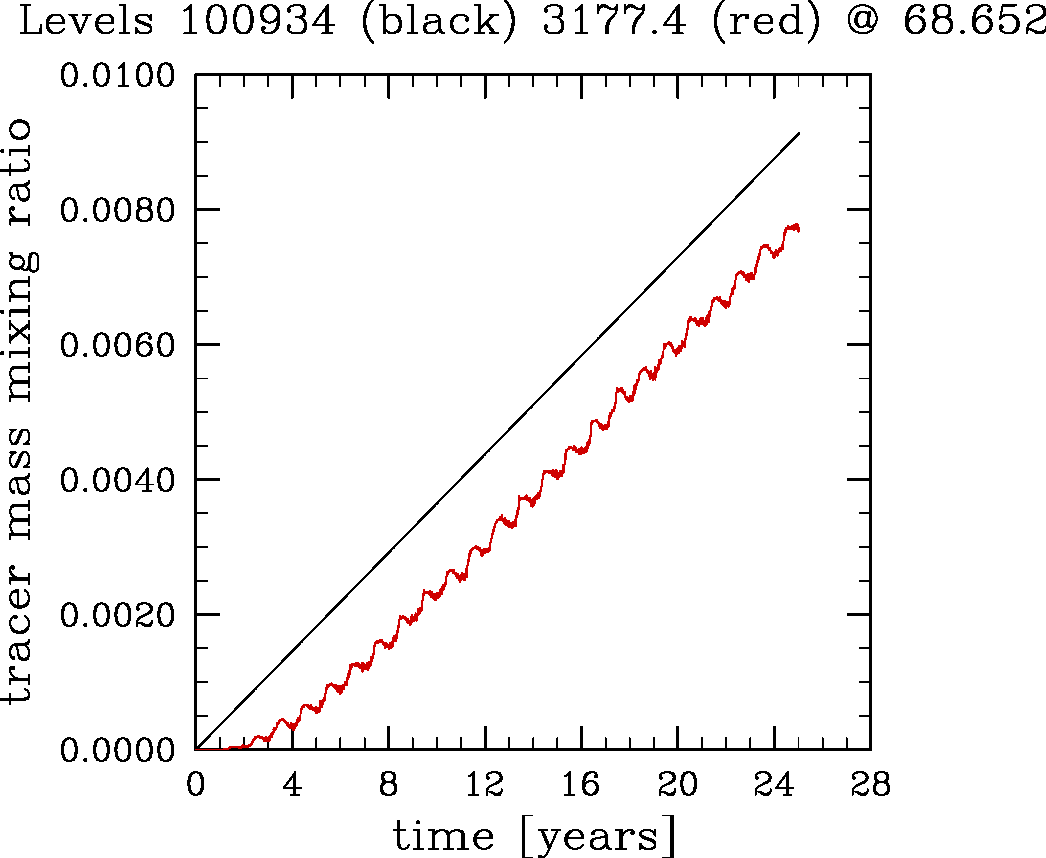
\includegraphics[width=12cm]{aoa_tracer_sample.pdf}
\igcrtwzeonfozefizenirjs{width=12cm}{aoa_tracer_sample.pdf}
\caption{The concentration of a passive tracer over time is shown at
  two different levels at $\approx 69^{\circ}$N in a model simulation
  performed with an early version of the ECHAM6 GCM under stationary
  present-day boundary conditions. The time lag between the
  concentrations can be used to derive the transport time of an air
  parcel from one grid point to the other and, thus, the age of
  air.}\label{fig_cr20140509rjs_aoa_tracer_sample} 
\end{figure}

Although the passive tracer is usually initialised at the surface, the
tropical tropopause is commonly used as the reference point for the
age of a stratospheric air parcel. As tracers are distributed rapidly
within the troposphere, the reference point can simply be set to a
certain location close to the tropical tropopause by subtracting the
tracer concentration at the reference grid point from any grid point
above. Following \cite{manzini1999} we use the 110 hPa level at the
equator as the reference grid point to calculate the age of air. The
zonal-mean age of air, obtained from all grid points above this
reference level in the 50-year present-day time-slice simulation with
ECHAM6, is shown in
Figure~\ref{fig_cr20140509rjs_age_of_air_sample}. The depicted age of
air distribution reflects the transport of air parcels along the
residual circulation trajectories in a coherent way. 

\begin{figure}
\centering
%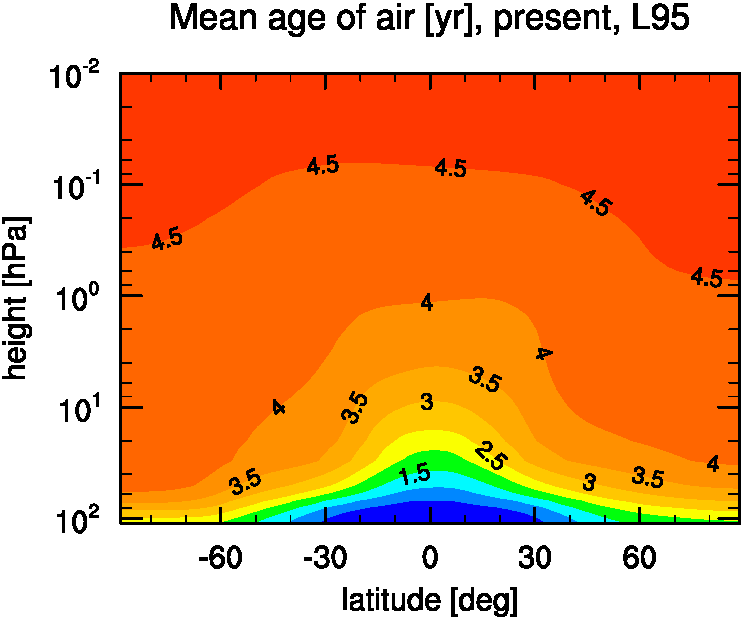
\includegraphics[width=12cm]{age_of_air_sample.pdf}
\igcrtwzeonfozefizenirjs{width=12cm}{age_of_air_sample.pdf}
\caption{The mean transit time of an air parcel originating from the
  tropical tropopause, i.e. the mean age of air, is shown. As in
  \cite{manzini1999}, the reference grid box is the 110 hPa level at
  the equator. The data represents the mean over the 50-year
  present-day time-slice simulation performed with the ECHAM6 GCM
  using 95 levels.}\label{fig_cr20140509rjs_age_of_air_sample} 
\end{figure}

Following \cite{hall1994} we derive the age spectrum of an air parcel
from a simulation of the spatio--temporal distribution of a tracer
that was injected into the atmosphere in a pulse. 
For a single time step the
mixing ratio of a passive tracer is set to 1 at every grid point
between -5 and +5 degrees latitude in the lowermost model
level. Before and after this time step the mixing ratio is forced to
zero at the same grid points. In this way the tracer concentration in
the injection grid points is as close as possible to Dirac's delta
distribution. Consequently, 
$n(P_0,t-t')$ can be substituted by $\delta(t-t_0)$ in
Equation~(\ref{eq_cr20140509rjs_green}) approximately,
leading to $G(P,P_0,t-t_0)=n(P,t)$. This shows that the age spectrum
$G(P,P_0,t-t_0)$ at any grid point $P$ is given by the tracer
concentration in that grid point. A certain amount of this tracer
pulse escapes the injection grid points between the injection and the
following time step. In order to normalise the age spectrum it is
divided by the total abundance of the tracer species left in the model
at the time step, at which the age spectrum is read out. To account
for seasonal differences in transport, one tracer pulse is injected on
January 1 and another one on July 1. Every 12 years tracer
concentrations are being reset, and a new pulse is injected. By
building the mean age spectrum of several tracer pulses, effects
originating from possible special atmospheric states can be
reduced. Figure~\ref{fig_cr20140509rjs_aoa_spectrum_sample} shows the
zonal-mean age spectrum of an air parcel at one grid point in the
high-latitude lower stratosphere in the 50-year present-day time-slice
simulation with ECHAM6, calculated by using the method described
above. The age spectrum peaks at roughly 2.5 years, while the long
tail of the spectrum reflects recirculated air parcels with an age of
up to the maximum age of 12 years (as tracer concentrations are being
reset after 12 years, see above). 

\begin{figure}
\centering
%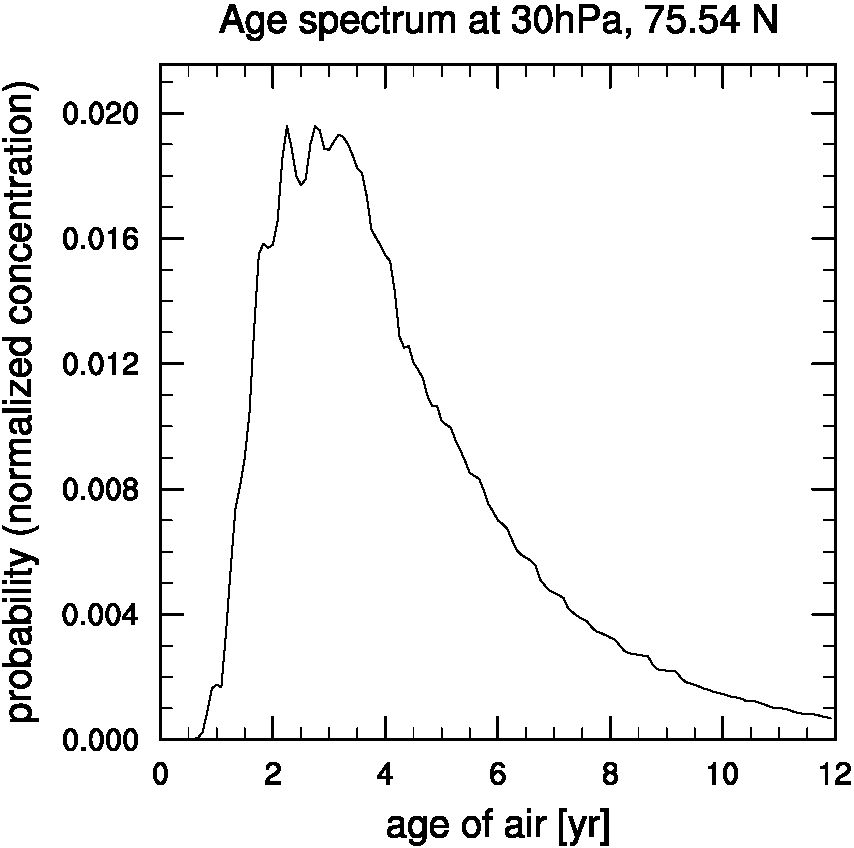
\includegraphics[width=12cm]{aoa_spectrum_sample.pdf}
\igcrtwzeonfozefizenirjs{width=12cm}{aoa_spectrum_sample.pdf}
\caption{The age spectrum of an air parcel located at 30 hPa and
  $75^{\circ}$N is shown. The data was derived from the 50-year
  present-day time-slice simulation performed with the ECHAM6 GCM
  using 95 levels.}\label{fig_cr20140509rjs_aoa_spectrum_sample} 
\end{figure}

\subsection{Implementation}

The age--of--air submodel consists of three passive tracers, one for
the mean age of air {\tt mean\_age}, and two that are used to
calculate the age spectra for winter and summer ({\tt spec\_winter},
{\tt spec\_summer}). 

\begin{description}
\item[{\tt init\_aoa}:] The age of air submodel consists of the 
subprograms {\tt init\_aoa},
{\tt bcond\_aoa}, {\tt get\_pointer2trac}, {\tt tracer\_reset}, and
{\tt tf\_reset} that are all collected in the module {\tt
  mo\_aoa.f90}. \newline
The subroutine {\tt init\_aoa} reads the namelist {\tt aoactl} 
from the file {\tt namelist.echam}, creates the tracers {\tt mean\_age},
{\tt spec\_winter}, and {\tt spec\_summer}, and sets the 
2--dimensional emission mask
{\tt emissions\_mask} to $1.0$ for each grid box where the tracers are
emitted, to $0$ where no emission takes place. Furthermore, the index
of the model level at which the emissions are injected into the
atmosphere is determined.
 
\item[{\tt bcond\_aoa}:]
Adds the emission rate to the tracer tendencies of {\tt mean\_age}, 
{\tt spec\_winter}, and {\tt spec\_summer}, respectively. The emission
rates are added only where {\tt emission\_mask} is larger than zero and
only if the model time lies in the appropriate time interval.
In the case of age--of--air tracers, the emission region is small 
compared to the globe and a {\tt where}--statement may be faster than 
a multiplication of the emission rate by {\tt emission\_mask}.

\item[{\tt get\_pointer2trac}:] This subroutine provides pointers to the 
3--dimensional fields hosting the mass mixing ratios of the tracers
{\tt mean\_age}, {\tt spec\_winter}, and {\tt spec\_summer} at
time step $t$ and $t-\Delta t$, respectively.

\item[{\tt tracer\_reset}, {\tt tf\_reset}:] 
The winter and summer tracer {\tt spec\_winter} and {\tt spec\_summer} 
have to be reset to zero after certain time intervals given
by the namelist in order to have good statistics in the determination
of the age spectrum. The program allows for a maximum number of
four re--initializations of these tracers. The variables
{\tt xt}, {\tt xtm1}, and {\tt pxtte} are reset in {\tt tracer\_reset},
the variable {\tt xtf} is reset in the {\tt tr\_reset}. The latter
variable occurs in the time filter and has to be reset also in order
to achive a complete re--initialization of the tracer.
\end{description}

\subsection{Usage}
\subsubsection{Namelist}
The age--of--air tracers controlled by the namelist {\tt aoactl}. 
It contains the following variables:

\setlength{\LTcapwidth}{\textwidth}
\setlength{\LTleft}{0pt}\setlength{\LTright}{0pt}

\begin{longtable}{l@{\extracolsep\fill}lp{6cm}l}\hline\hline
\caption[Namelist aoactl]{Namelist {\tt aoactl}}\\\hline
\label{tab_cr20140509_aoactl}
\endfirsthead
\caption[]{aoactl --- continued}\\\hline
\endhead
\hline\multicolumn{2}{r}{\slshape table continued on next page}\\
\endfoot
\hline %\multicolumn{2}{r}{end of table}
\endlastfoot
Variable & Type & Explanation & Default\\\hline
{\tt conc\_increase} & double prec. & increase of {\tt mean\_age} tracer
in mass mixing ration per day. The mass mixing ratio in the region where
${\tt emission\_mask} > 0$ is ${\tt conc\_increase}\times t$ after time $t$. 
& {\tt 1.0e-6\_dp}\\
{\tt dt\_start\_emi\_summer\_1} & integer(6) & year, month, day, hour, minute, 
second of first time that the emission of the tracer {\tt spec\_summer} starts.
The emission lasts one time step only. The date should be in summer. 
& {\tt 1978,1,2,0,0,0}\\
{\tt dt\_start\_emi\_summer\_2} & integer(6) & year, month, day, hour, minute, 
second of second time that the emission of the tracer 
{\tt spec\_summer} starts.
The emission lasts one time step only. The date should be in summer and about 
12~years after {\tt dt\_start\_emi\_summer\_1}. & {\tt 1990,1,2,0,0,0}\\
{\tt dt\_start\_emi\_summer\_3} & integer(6) & year, month, day, hour, minute, 
second of third time that the emission of the tracer 
{\tt spec\_summer} starts.
The emission lasts one time step only. The date should be in summer and about 
12~years after {\tt dt\_start\_emi\_summer\_2}. & {\tt 2002,1,2,0,0,0}\\
{\tt dt\_start\_emi\_summer\_4} & integer(6) & year, month, day, hour, minute, 
second of second time that the emission of the tracer 
{\tt spec\_summer} starts.
The emission lasts one time step only. The date should be in summer and about 
12~years after {\tt dt\_start\_emi\_summer\_3}. & {\tt 2014,1,2,0,0,0}\\
{\tt dt\_start\_emi\_winter\_1} & integer(6) & year, month, day, hour, minute, 
second of first time that the emission of the tracer {\tt spec\_winter} starts.
The emission lasts one time step only. The date should be in winter. 
& {\tt 1978,1,2,0,0,0}\\
{\tt dt\_start\_emi\_winter\_2} & integer(6) & year, month, day, hour, minute, 
second of second time that the emission of the tracer 
{\tt spec\_winter} starts.
The emission lasts one time step only. The date should be in winter and about 
12~years after {\tt dt\_start\_emi\_winter\_1}. & {\tt 1990,1,2,0,0,0}\\
{\tt dt\_start\_emi\_winter\_3} & integer(6) & year, month, day, hour, minute, 
second of third time that the emission of the tracer 
{\tt spec\_winter} starts.
The emission lasts one time step only. The date should be in winter and about 
12~years after {\tt dt\_start\_emi\_winter\_2}. & {\tt 2002,1,2,0,0,0}\\
{\tt dt\_start\_emi\_winter\_4} & integer(6) & year, month, day, hour, minute, 
second of second time that the emission of the tracer 
{\tt spec\_winter} starts.
The emission lasts one time step only. The date should be in winter and about 
12~years after {\tt dt\_start\_emi\_winter\_3}. & {\tt 2014,1,2,0,0,0}\\
{\tt emission\_lat\_n} & double prec. & latitude of the northern boundary of the emission 
region in degrees north& $5^\circ$ \\
{\tt emission\_lat\_s} & double prec. & latitude of the southern boundary of the emission 
region in degrees north& $-5^\circ$ \\
{\tt emission\_plev} & double prec. & Pressure level of emission in hPa. More 
precisely, the emission is injected in the model level with the
lowest pressure at the midpoint of which the
pressure at the lower boundary is larger than {\tt emission\_plev}. 
The pressure of the model levels are determined using a surface pressure
of $101325\,{\rm Pa}$. & $1013.25\,{\rm hPa}$\\
\hline
\end{longtable}
 
\subsubsection{Postprocessing}
There are two ncl--scripts provided at \newline
{\tt https://svn.zmaw.de/svn/diagnostics/trunk/diagnostics/echam/}
\newline
that create 
graphical output of the age of air calculated from the tracer output 
of the age--of--air submodel. The {\tt contour\_age.ncl} script 
creates a contour plot with the mean age of air from the {\tt mean\_age}
tracer, {\tt aoa\_spectrum.ncl} calculates the age spectrum of air at
a certain model level and latitude.

\paragraph{contour\_age.ncl:} This script requires yearly files with 
monthly means, but it can calculate the zonal mean by itself. There are 
lines at the beginning of the ncl--script that have to be adjusted to 
the actual experiment.
\setlength{\LTcapwidth}{\textwidth}
\setlength{\LTleft}{0pt}\setlength{\LTright}{0pt}
\begin{longtable}{l@{\extracolsep\fill}p{9cm}}\hline\hline
\caption[Variables of contour\_age.ncl]
{Variables of {\tt contour\_age.ncl}}\\\hline
\label{tab_cr20140509_contourage}
\endfirsthead
\caption[]{contour\_age --- continued}\\\hline
\endhead
\hline\multicolumn{2}{r}{\slshape table continued on next page}\\
\endfoot
\hline %\multicolumn{2}{r}{end of table}
\endlastfoot
\hline
Variable & Explanation \\\hline
{\tt cdo\_cmd} & cdo--command that will be executed before the mean
age is calculated, e.g. {\tt ``zonmean''} for the calculation of zonal
mean values, or {\tt ``zonmean -monmean''} to calculate monthly means
and zonal means.\\
{\tt climean} & period of time over which the monthly means are averaged,
e.g. {``YEAR''}, {``DJF''}, or {``JJA''}.\\
{\tt datdir} & path of input files\\
{\tt dstring} & Plot title\\
{\tt expm} & infix of input files describing the experiment, e.g. 
{\tt ``DEV0107''}\\
{\tt emission\_start}& start year of emissions\\
{\tt first\_year} & first year from which the global tracer increase
can be considered to be linear.\\
{\tt fname\_suffix} & suffix of \echam{} input files. In most cases either 
{\tt ``tracer''} or {\tt ``tracerm''}\\
{\tt last\_year} & last year that will be used in the age--of--air 
calculation\\
{\tt lat\_idx\_n} & index of northern latitude up to which the age
of air is calculated. It has to be counted from the equator. E.g. 46
in the case of a horizontal resolution T63.\\
{\tt lat\_idx\_s} & index of southern latitude up to which the age of air is
calculated. It has to be counted from the equator, E.g. 47 in the 
case of a horizontal resolution T63.\\
{\tt proj} & will be a part of the ourput filename, e.g. {\tt ``SHARP''}\\
{\tt reflevel} & pressure in hPa at which the age of air is 
defined to be zero. Usually, {\tt relevel=11000}, i.e.~ the age 
of air is assumed to be zero at $110\,{\rm hPa}$. \\
{\tt wks\_type} & format of graphics output, e.g. {\tt ``eps''}\\
\end{longtable}

\paragraph{aoa\_spectrum.ncl:} This script requires yearly files with 
monthly means of the pulsed tracers {\tt spec\_winter} and 
{\tt spec\_summer}. There are 
lines at the beginning of the ncl--script that have to be adjusted to 
the actual experiment.
\setlength{\LTcapwidth}{\textwidth}
\setlength{\LTleft}{0pt}\setlength{\LTright}{0pt}
\begin{longtable}{l@{\extracolsep\fill}p{9cm}}\hline\hline
\caption[Variables of aoa\_spectrum.ncl]
{Variables of {\tt aoa\_spectrum.ncl}}\\\hline
\label{tab_cr20140509_aoaspectrum}
\endfirsthead
\caption[]{aoa\_spectrum --- continued}\\\hline
\endhead
\hline\multicolumn{2}{r}{\slshape table continued on next page}\\
\endfoot
\hline %\multicolumn{2}{r}{end of table}
\endlastfoot
\hline
Variable & Explanation \\\hline
{\tt datdir} & path of input files\\
{\tt cdo\_cmd} & cdo--command that will be executed before the mean
age is calculated, e.g. {\tt ``zonmean''} for the calculation of zonal
mean values, or {\tt ``zonmean -monmean''} to calculate monthly means
and zonal means.\\
{\tt emission\_years} & time interval between emission pulses in years\\
{\tt expm} & infix of input files describing the experiment, e.g. 
{\tt ``DEV0107''}\\
{\tt first\_emissions} & year of first emission pulse\\
{\tt fname\_suffix} & suffix of \echam{} input files. In most cases either 
{\tt ``tracer''} or {\tt ``tracerm''}\\
{\tt latidx} & index of latitude at which age spectrum is to be calculated\\
{\tt levidx} & index of level at which age spectrum is to be calculated\\
{\tt no\_of\_trac} & total number of emission pulses\\
{\tt proj} & will be a part of the ourput filename, e.g. {\tt ``SHARP''}\\
{\tt wks\_type} & format of graphics output, e.g. {\tt ``eps''}\\
\hline
\end{longtable}
%\begin{lstlisting}
%code
%\end{lstlisting}

